\documentclass[tikz,border=10pt]{standalone}

\begin{document}

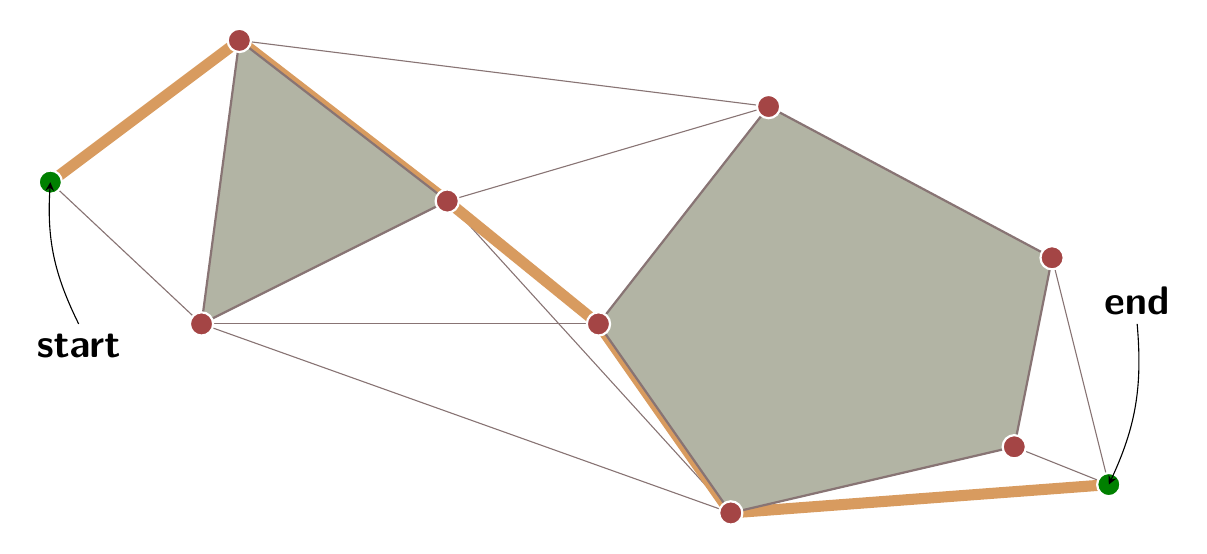
\begin{tikzpicture}[scale=1.2, line join=round]

    % --- Colors matching the Stanford graphics ---
    \definecolor{polyfill}{RGB}{178, 180, 164}
    \definecolor{polyborder}{RGB}{136, 116, 116}
    \definecolor{nodefill}{RGB}{164, 69, 69}
    \definecolor{startend}{RGB}{0, 128, 0}
    \definecolor{pathcolor}{RGB}{216, 155, 95}

    % --- Coordinates ---
    \coordinate (start) at (0, 4);
    
    % Triangle coordinates
    \coordinate (t1) at (2, 5.5);
    \coordinate (t2) at (1.6, 2.5);
    \coordinate (t3) at (4.2, 3.8);
    
    % Pentagon coordinates
    \coordinate (p1) at (5.8, 2.5);
    \coordinate (p2) at (7.6, 4.8);
    \coordinate (p3) at (10.6, 3.2);
    \coordinate (p4) at (10.2, 1.2);
    \coordinate (p5) at (7.2, 0.5);
    
    \coordinate (end) at (11.2, 0.8);


    % --- 1. Draw Visibility Edges (Underneath everything) ---
    % Notice the trailing comma at the very end of the list to prevent whitespace errors
    \foreach \u/\v in {
        start/t1, start/t2,
        t1/p2, t1/t3, t1/p1,
        t2/p1, t2/p5, t2/t3,
        t3/p1, t3/p2, t3/p5,
        p2/p3, p3/p4, p4/p5, p5/p1, p1/p2,
        p3/end, p4/end, p5/end%
    } {%
        \draw[polyborder, thin] (\u) -- (\v);%
    }

    % --- 2. Draw the Highlighted Path ---
    \draw[pathcolor, line width=4pt] (start) -- (t1) -- (t3) -- (p1) -- (p5) -- (end);

    % --- 3. Draw Polygons ---
    \filldraw[fill=polyfill, draw=polyborder, thick] (t1) -- (t2) -- (t3) -- cycle;
    \filldraw[fill=polyfill, draw=polyborder, thick] (p1) -- (p2) -- (p3) -- (p4) -- (p5) -- cycle;

    % --- 4. Draw Nodes ---
    \foreach \n in {t1, t2, t3, p1, p2, p3, p4, p5} {
        \filldraw[nodefill, draw=white, thick] (\n) circle (3.5pt);
    }

    \foreach \n in {start, end} {
        \filldraw[startend, draw=white, thick] (\n) circle (3.5pt);
    }

    % --- 5. Labels and Arrows ---
    % Start label
    \node[font=\sffamily\bfseries\Large, anchor=north] (lstart) at (0.3, 2.5) {start};
    \draw[-stealth, thin] (lstart.north) to[bend left=15] (start);

    % End label
    \node[font=\sffamily\bfseries\Large, anchor=south] (lend) at (11.5, 2.5) {end};
    \draw[-stealth, thin] (lend.south) to[bend left=15] (end);

\end{tikzpicture}

\end{document}